\section{Motivation}
\label{sec:motivation}
% TODO(main): basis — motivation on upstream tree, evaluation on pinned tree; align before submission
% Sources (Part 4, read-only): 00_doc/vortex-wgdxa2k/results/MOTIVATION_MASTER.md (reference core, 55 variants),
% MOTIV_MASTER_FQ16.md sections 2 and 5b (tuning chain, binding limits), MOTIV_MASTER_TC_TABLES.md sections B, F, G, I
% (tuned core: MACs per instruction, register reads, loads, GEMV). Figure data and asserts: fig/src/motiv_simt.py.

% P:mot-setting
We characterize GEMM and decode GEMV on SIMT-only Vortex, the same core with its tensor core switched off, to find the inefficiencies a tensor core must remove. The reference core runs four warps of 8 threads and issues one warp instruction per cycle, so its 8 FP32 lanes peak at 16~FLOP per cycle. Each kernel is the fastest of 55 SIMT variants rather than a naive loop; the variants differ in register tile, thread-block shape, $K$ tile and staging through shared memory. Even so, the best $128{\times}128{\times}512$ GEMM reaches only 17\% of the peak. We first remove the limits that a SIMT design can tune away, which gives a tuned baseline, and then measure on that baseline four inefficiencies that tuning leaves in place: work per instruction, register-file reads, load granularity and the bytes of decode GEMV.
% TODO(part4-owner): "55 variants" is MOTIVATION_MASTER.md sections 0 and 2; MOTIV_MASTER_FQ16.md section 6 item 4 counts 45 at the NW 4 reference -- confirm the count.

\begin{figure}[t]
    \centering
    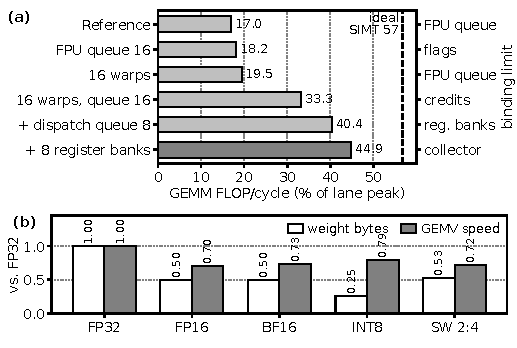
\includegraphics[width=\columnwidth]
    {hpca2027-latex-template/fig/motiv_simt.pdf}
    \caption{SIMT-only Vortex: (a)~GEMM share of the lane peak as limits are removed, and the limit that then binds; (b)~decode-GEMV weight bytes and speed by format, relative to FP32.}
    \label{fig:motiv_simt}
\end{figure}

% P:mot-tuned-baseline
\textbf{Tuned baseline.} Four limits of the reference core are microarchitectural, and a SIMT design removes or hides each by sizing its core (Fig.~\ref{fig:motiv_simt}(a)). The FPU queue admits two instructions per FPU and holds each until its result leaves the FPU. Every floating-point instruction writes the warp's exception-flags register, so the scoreboard lets a warp keep only one such instruction in flight, and only more warps hide this ordering. Dispatch credits cap the instructions queued for each functional unit. The register file has four banks that serve one operand each per cycle, so an instruction whose sources share a bank waits in the operand collector. Raising the warp count to 16 and removing the other limits in turn, with a 16-entry FPU queue, an 8-entry dispatch queue and 8 register banks, lifts the GEMM from 17\% to 45\% of the peak. Even an ideal SIMT pipeline that issues one warp instruction every cycle would stop at 57\%, a cap that the instruction mix sets. The tuned core is the baseline for the rest of this section.
% TODO(main): the evaluation's SIMT baseline (sec:eval_threads, "scalar FP32 execution at the same thread count", Table tab:config) is not this tuned core (FPU queue 16, dispatch queue 8, 8 GPR banks); MOTIVATION_PAGE_PLAN.md section 4 asks the evaluation to adopt it.

% P:mot-work-per-instr
\textbf{Work per instruction.} A SIMT instruction performs at most one multiply-accumulate (MAC) per lane, so the threads per warp cap the work of every instruction. A fused multiply-add (FMA) instruction reaches this cap, whereas loads, address arithmetic and loop control perform no MAC. The tuned GEMM therefore averages 4.5 MACs per warp instruction against the 8 of an FMA, and this mix sets the 57\% cap. A SIMT core raises its peak only by adding lanes or issue slots, and each brings the same instruction mix.

% P:mot-register-reads
\textbf{Register-file reads.} Every MAC of a SIMT kernel reads its operands from the register file: a thread-level FMA reads three registers for one MAC, the operands $a$ and $b$ and the accumulator $c$. A larger thread tile reuses each loaded value for more MACs and so cuts memory loads, but it leaves the three reads of each FMA unchanged. With its loads and address instructions, the tuned GEMM reads 3.9 registers per MAC. In a register file of four banks, FMAs cause almost all of the bank conflicts.

% P:mot-load-granularity
\textbf{Load granularity.} A SIMT load moves one element into the register of one lane, so operands enter the register file one element per lane per instruction. The tuned GEMM issues one load or store instruction for every 13 MACs, and loads and stores make up a third of its instructions. A value that every lane of a warp needs, such as the element of $A$ that each lane multiplies by its own column of $B$, is loaded into every lane, so many loaded words are copies of one value. Staging tiles through shared memory does not remove these loads: it replaces global loads with shared-memory loads and adds stores, address arithmetic and barriers, and the fastest kernels load directly from global memory.

% P:mot-gemv-bytes
\textbf{Bytes in decode GEMV.} Decode GEMV uses each weight once, so fewer bytes per weight are its only lever, and SIMT cannot turn fewer bytes into speed. We run the batch-1 GEMV of an $8192{\times}2048$ feed-forward layer of Llama-3.2-1B. A SIMT FMA takes one FP32 value per register, so FP16 weights need a load and a conversion per element, INT8 weights a byte load and integer arithmetic, and software 2:4 sparsity index arithmetic to fetch the input element that each kept weight multiplies. These formats store a weight in a quarter to about half of its FP32 bytes, yet on the tuned core they run at only 0.7--0.8$\times$ the FP32 speed (Fig.~\ref{fig:motiv_simt}(b)).
% TODO(main): weight bytes are the storage size; the measured DRAM bytes on the tuned core are 0.95/0.69/0.29/0.56x FP32 for FP16/BF16/INT8/software 2:4 (MOTIV_MASTER_TC_TABLES.md section I, "SIMT gpr8" rows), so FP16 barely cuts DRAM traffic there.

% P:mot-common-cause
The four inefficiencies share one cause: the unit of SIMT work is one scalar MAC per lane. A tensor core makes the unit a tile operation, on operands held across the registers of a warp for warp-level MMA or read from shared memory by a warpgroup for warp-group MMA, so each instruction, register read and load feeds many MACs, and narrow formats enter its datapath without conversion. Compressed weights also need hardware that consumes them, which a 2:4 sparse tensor core provides. FourShadow builds these tensor cores into Vortex (Section~\ref{sec:design}), and the evaluation varies the parameter behind each inefficiency: threads per warp and issue width for the work per instruction (Sections~\ref{sec:eval_threads} and~\ref{sec:eval_iw}), accumulator registers for the register reads (Section~\ref{sec:eval_nrc}), shared-memory operand staging for the loads (Sections~\ref{sec:bg_smem} and~\ref{sec:eval_delay_a}), and 2:4 sparsity for the bytes (Section~\ref{sec:eval_sparse}).
% TODO(main): promise gaps from MOTIVATION_PAGE_PLAN.md section 4 -- no SIMT-baseline MACs-per-instruction comparison in sec:eval_threads, no WGMMA+/-DXA load counts, no decode-shape (GEMV) sparse tensor-core result in sec:eval_sparse.
